\section{Introduction}
The elasticity of cloud computing has changed 
the way resources are managed and allocated. 
Cloud computing provides a management interface 
for a large pool of resources and brings different 
services to users (IaaS, PaaS, SaaS). With its 
promising success in industry, cloud computing has become a 
 hot research topic. Despite its popularity in research 
 communities, cloud computing infrastructures are either 
 proprietary or depend on softwares that are closed and 
 impossible to instrument. This prevents researchers from 
having the power to innovate and develop new ideas in cloud computing.\\
Eucalyptus~\cite{nurmi2009eucalyptus} is an open and modular cloud computing platform that 
allows researchers to instrument, modify, and realizes different 
research ideas in cloud computing. Eucalyptus provides a well-define API 
that are compatible with industry (Amazon EC2 and S3) and allow 
researchers to try new components. Eucalyptus is also easy to deploy 
on existing resources.\\
The goal of this lab assignment is to install a simple working set of 
Eucalyptus on commodity hardware (Emulab~\cite{white2002integrated} testbed machines). 
The installed Eucalyptus should include 
a cloud controller (CLC), a cluster controller (CC), and a node controller (NC). 
The system administrator is able to manage resources: create instances using different 
OS images or remove an instances. Users are able to log in and use the instances. 
The system operates in a static network mode in which the administrator 
has to specify the network configuration that each instance will receive from 
the DHCP server that runs on the cluster controller of the instance. 


\section{Installation and screen shoots}
\begin{enumerate}
	\item Hardware and topology: the installation hardware 
		consists of 3 physical machines in Emulab testbed. 
		The 3 machines are able to run VMs and connect to 
		each other in a VLAN. Each machine (node) hosts one of the 3 
		components separately: CLC, CC, and NC. They are accessible via public 
		IP addresses.
	\item Install Eucalyptus: This experiment installs Eucalyptus 
		from release packages. Eucalyptus, Euca2ools, and EPEL 
		are installed on every node while software is installed 
		corresponding to the functionality of a node: cloud controller 
		software runs on CLC, cluster controller software runs on 
		CC, and node controller software runs on NC. Walrus is 
		hosted by CLC (although it could be hosted separately).
	\item Network Configuration:\\
		Since the interfaces of the image used in the experiment 
		(CENTOS64-64) is not configured by Emulab, network-scripts are created 
		and added to /etc/sysconfig/network-scripts/ manually. The 3 nodes 
		then connected via the defined interfaces and are able to ping each 
		other.\\
		CC runs a DHCP server that assigns IP for 
		any instance that run on NC nodes underneath. In static network mode, 
		the MAC-IP mapping inside DHCP server is explicitly specified. DHCP configuration 
		is done by specifying parameters in /etc/eucalyptus/eucalyptus.conf file 
		(this file also determines the storage/network/virtualization options on each node). 
		For example, if the MAC-IP in this setup is specified as
		\textit{"AA:BB:CC:DD:EE:FF=10.1.1.11"}, the new instance will get the IP 
		\textit{10.1.1.11} when it boots up.\\
		Eucalyptus uses the eucalyptus.conf file to create the real configuration file 
		that is actually used by the dhcp server (the file locates in /var/run/eucalyptus/net). 
		A log of network configuration when CC starts is shown in screen shoot ~\ref{fig:cc_network}. 
		screen shoot ~\ref{fig:dhcp_daemon} shows the dhcp server daemon running on CC node.
		\begin{figure}[hbtp]
			\centering
			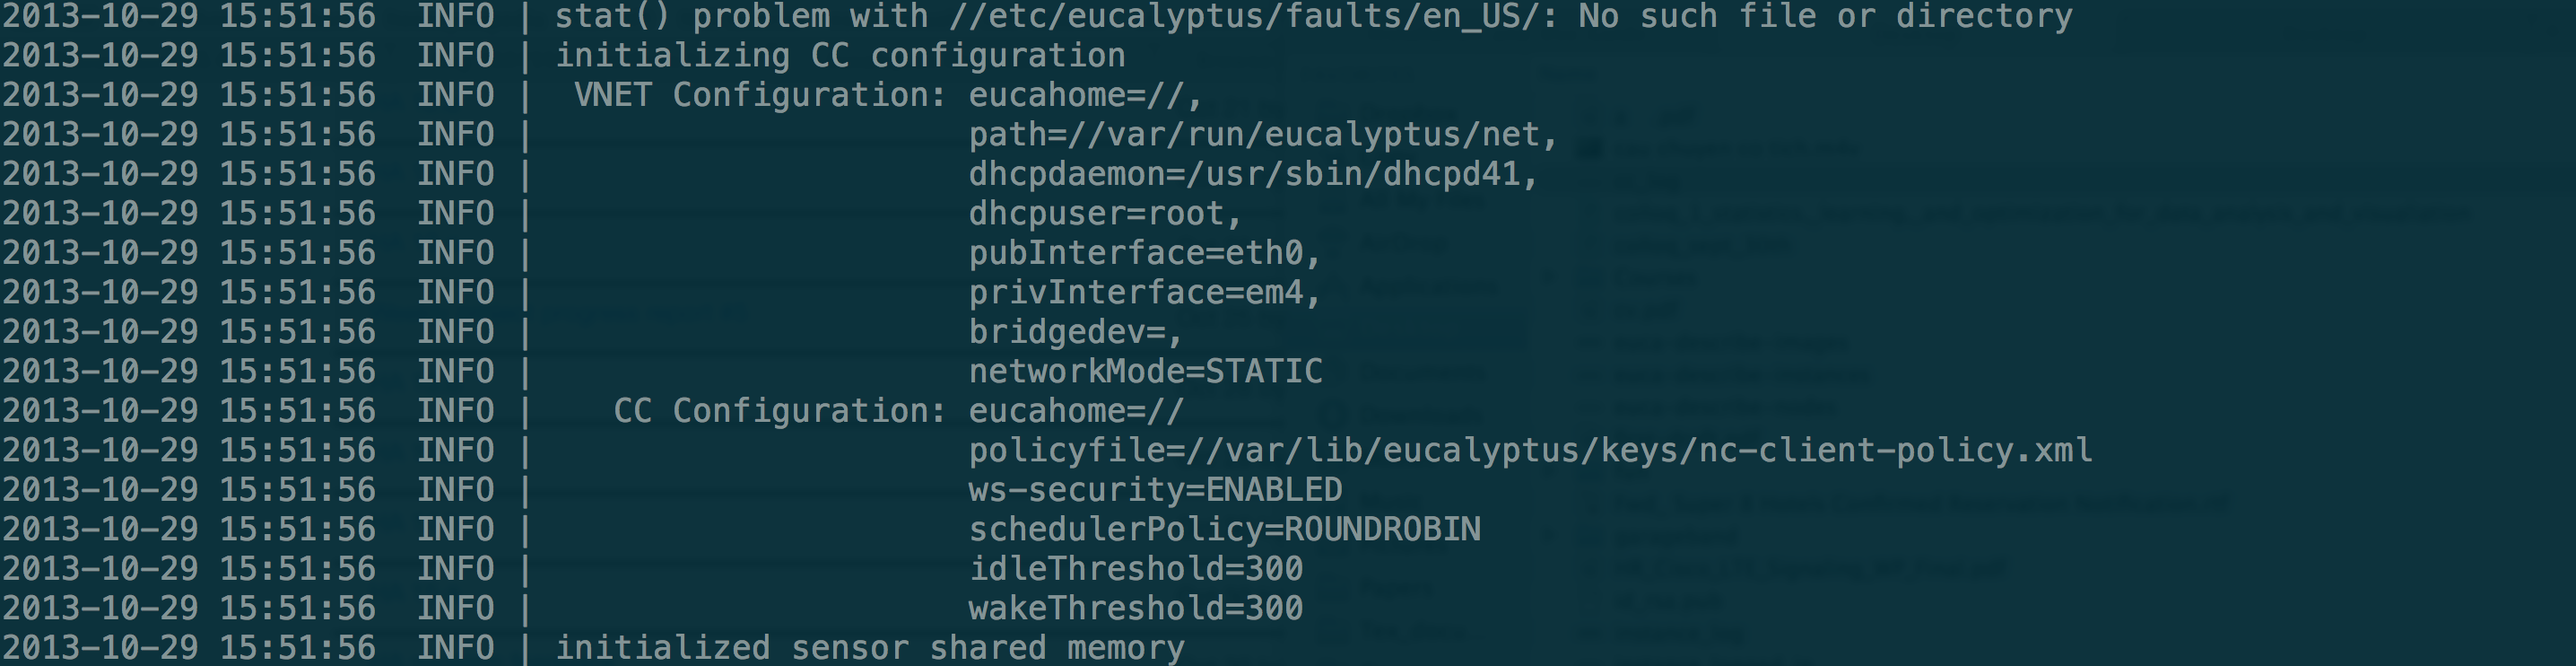
\includegraphics[scale=0.14]{cc-network.png}
			\caption{ Configuration log on CC node.
			}
			\label{fig:cc_network}
		\end{figure}

		\begin{figure}[hbtp]
			\centering
			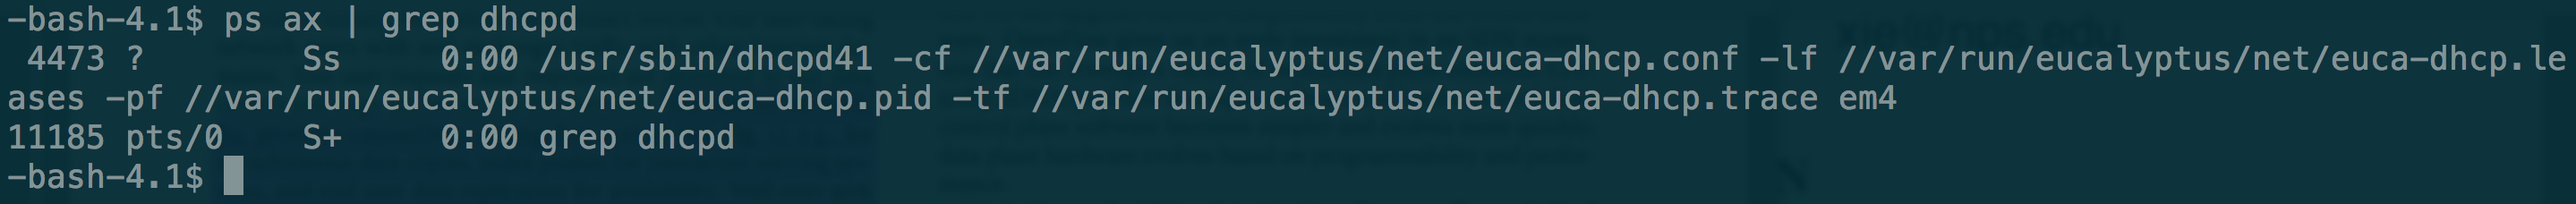
\includegraphics[scale=0.14]{dhcp-daemon.png}
			\caption{ DHCP daemon is running on CC node
			}
			\label{fig:dhcp_daemon}
		\end{figure}
	\item Register and start Walrus, CC, and NC: Walrus and CC are registered on the CLC node 
		that controls them while NC is registered on the CC node of the same 
		control domain. After registering these components, the NC is able to start. 
		The CC is able to see the status of all NCs underneath by using \textit{"euca-describe-nodes"} 
		command ( as in screen shoot ~\ref{fig:describe_nodes}).
		\begin{figure}[hbtp]
			\centering
			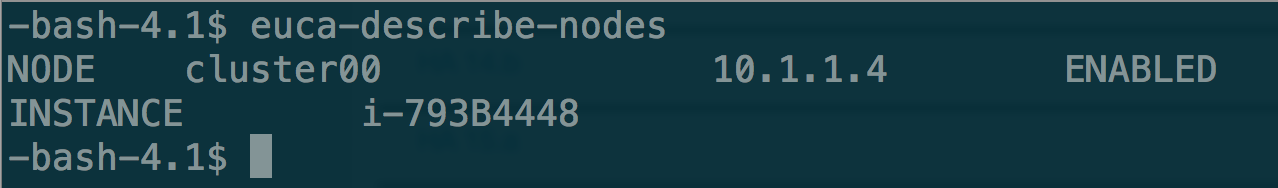
\includegraphics[scale=0.3]{describe-nodes.png}
			\caption{ CC node shows all enabled nodes}
			\label{fig:describe_nodes}
		\end{figure}
	\item Download image from Eustore and launch instance:\\
		To access to Eustore, a admin credential is used. The credential 
		is created by running 
		\textit{"/usr/sbin/euca\_conf --get-credentials"}. After creating the 
		admin credential, the operator loads credential information by  
		running \textit{"source eucarc"}. After that, the operator is able to
		download images from Eustore using image ID. 
		Operator also have to create keypairs that 
		are used for accessing instances.\\
		After having an image downloaded, operator can launch an instance on the 
		NC and specify the keypair that is used to access that instance. 
		The keypair consists of a public and a private key. While the public key 
		is uploaded to CLC and associated with the target instance, cloud user uses private key 
		to access the instance that has the corresponding public key.
		A successfully launched instance is described as in 
		screen shoot ~\ref{fig:describe_instances}.
		\begin{figure}[hbtp]
			\centering
			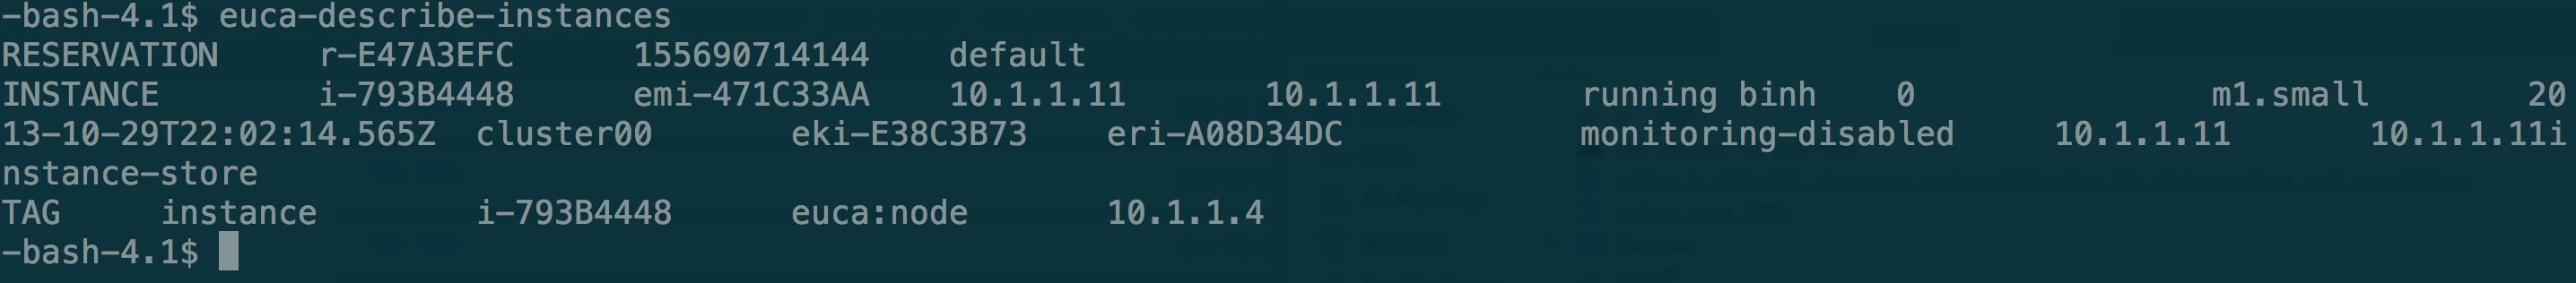
\includegraphics[scale=0.15]{describe-instances.png}
			\caption{ The instance running on NC. The key associated 
				with the instance named \textit{binh}, the IP address 
				of the instance is \textit{10.1.1.11}, instance ID is 
				\textit{i-793B4448}.
			}
			\label{fig:describe_instances}
		\end{figure}
		Routing information for the instance could be found in the 
		console output of a running instance (obtained by \textit{euca-get-console-output <instance ID>}). 
		The log shows the network configuration during booting (as in ~\ref{fig:instance_log}).
		\begin{figure}[hbtp]
			\centering
			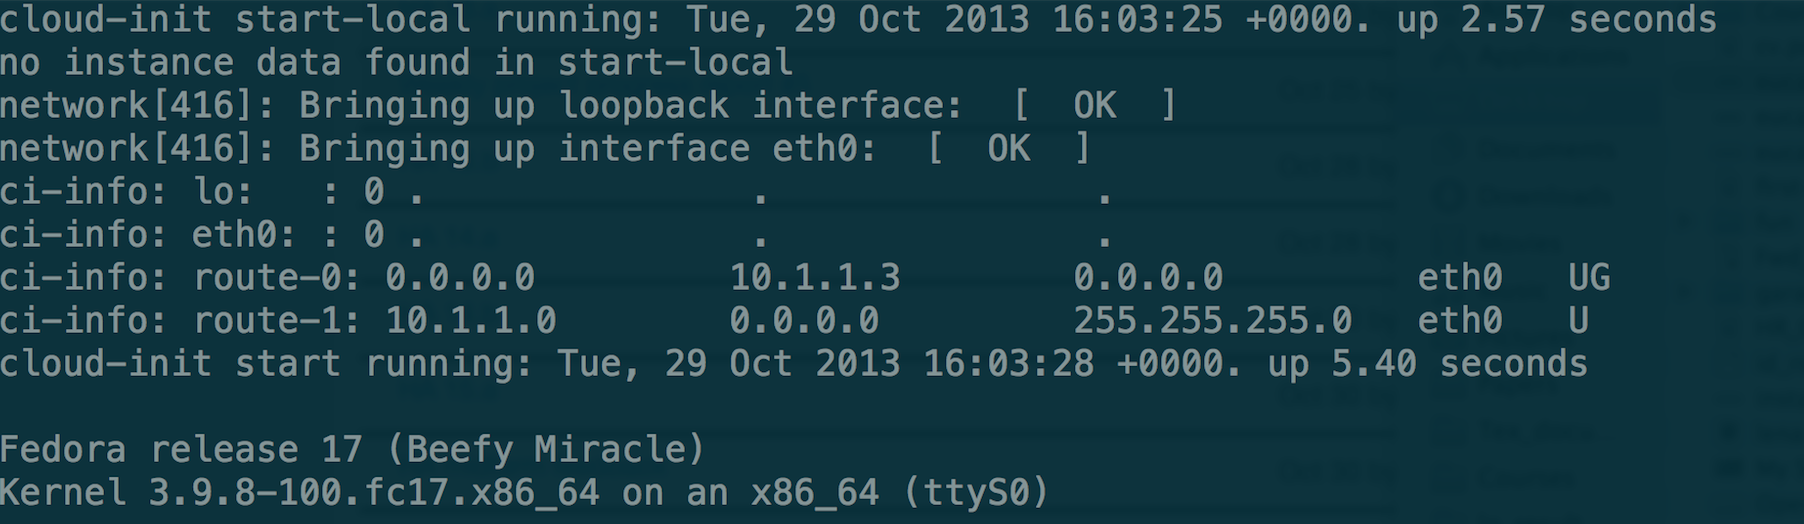
\includegraphics[scale=0.23]{instance-log.png}
			\caption{ Interface starting up in the instance.
			}
			\label{fig:instance_log}
		\end{figure}
	\item Log into the instance using the keypair: a cloud user can 
		login and use the instance that is running. The screen shoot 
		~\ref{fig:login} shows the login command. Cloud user successfully 
		logged into the instance using the private key and gained the 
		root privilege. 
		\begin{figure}[hbtp]
			\centering
			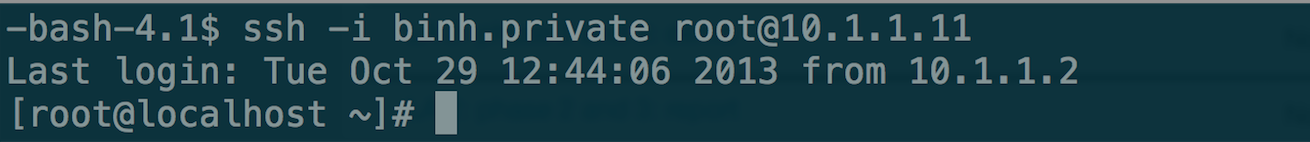
\includegraphics[scale=0.35]{login.png}
			\caption{ Cloud user accesses the instance using the associated private key
			}
			\label{fig:login}
		\end{figure}
\end{enumerate}


\section{Conclusion}
In this lab assignment, a simple but complete set of Eucalyptus was successfully 
installed on three physical machines. Operators can manage 
images/instances and provide the resources to cloud users. Although the 
installation process is specified in Eucalyptus documents, different system modes 
require different installation steps/requirements. The entire installation 
process is automated and repeatable using bash scripts. The detailed 
scripts could be found \href{https://github.com/binhqnguyen/cs6480}{here}. 


